\chapter{Trend Analysis}\label{ch:TA}
\section{Methods}
\subsection{Introduction}

Trend analysis is a great way to characterize the park's water quality using data collected through the stream survey. It is used to state the condition of the parks water bodies while trying to predict where the water quality is headed in the future. A trend analysis on the stream survey data was conducted in 2002 and published in \citet{robinson2008ph} and then again in 2009 for the Biotics Effects report \citep{cai2012}. This statistical procedure is used to discover sudden and gradual trends over time. Of the ten elevation bands analyzed in \citet{robinson2008ph} six had negative Julian date coefficients and the other four had no trend. Of the 67 sites studied in the biotic effects report most showed no trend, 22 showed an increase in pH and 2 showed a decrease\citep{cai2012}. The trend analysis will use stream survey data from 1993 to 2012 using the statistical programs JMP and SPSS for analysis.

\subsection{Body}

Water quality is an ongoing concern for the park. The acidification of the streams can have significant negative effects on wildlife and vegetation. The stream survey collects water samples all over the park to monitor the health of the water. 
    
 The data used in these analyses are collected through the park wide stream survey. The stream survey includes six stream systems and five of them are collected every two months and analyzed in a lab for many water quality variables including pH, ANC, NO$_3^-$, SO$_4^{2-}$ and some metals.  Hazel stream system %description of lab process in Intro?
The stream survey water quality data includes measurements for pH, ANC, conductivity, acid anions (CL$^-$,SO$_4^{2-}$,NO$_3^-$, ammonia (NH$_4^+$), the base cations (Ca$^{2+}$, Mg$^{2+}$, K$^+$, and Na$^+$), dissolved metals (Al, Cu, Fe, Mn, Si and Zn).  A ManTech$^{TM}$ autotitrator was used for pH, ANC, and conductivity.  A Dionex$^{TM}$ ion chromatograph (IC) was used for the analysis of CL$^-$, SO$_4^{2-}$, NO$_3^-$, and NH$_4^+$.  A Thermo-Scientific$^{TM}$ Inductively Coupled Plasma - Atomic Emission Spectrometry (ICP-AES) was used for the study of Ca$^{2+}$, Mg$^{2+}$, Na$^+$, K$^+$, Al, Cu, Fe, Mn, Si and Zn.

Twenty years of data were available for this paper from the years 1993 to 2012.  A single trend line containing all 20 years is unrealistic because it will not show why there is a difference in the previous trend analyses or if there was a change in trend after 2008. The opposite trends reported in  \citet{robinson2008ph} and \citet{cai2012} suggest an inflection point in the trend line somewhere between 2002 and 2009. For this reason, and for easier comparison of results,  a separate data set will be sectioned off from 1993 to 2002 to equal the years analyzed in \citet{robinson2008ph}. A third data set will be created after the year 2008 because this is the year that the Kingston and Bull run power plants installed scrubbers onto their smoke stack exhaust. The hypothesis being the SO$_4^{2-}$ concentrations will be noticeably different, and this difference could indicate a need for further study. These three time sets will be analyzed separately.

\begin{table}[htbp]
\caption{These elevation classes were created to add more weight to the higher elevations}
\begin{tabular}{clcp{5cm}}
\toprule
Elevation Classes & Meters (Feet)                              & n & Site \# \\ 
\midrule
1                        & 304.8-609.6 (1000-2000)           & 5   & 13 ,23, 24, 30, 479 \\ 
2                        & 609.6-762 (2000-2500)              & 9   & 4, 311, 268, 480, 310, 483, 147, 148, 484 \\ 
3                        & 762-914.4 (2500-3000)              & 13 & 114, 481, 482, 149, 66, 492, 137, 293, 270, 493, 485, 144, 224 \\ 
4                        & 914.4-1066.8 (3000-3500)         & 4   & 143, 142, 73, 71 \\ 
5                        & 1066.8-1371.6 (3500-4500)       & 4   & 74, 221, 251, 233 \\ 
6                        & $1371.6< (4500<)$                    & 2   & 253, 234 \\ 
\bottomrule
\end{tabular}
\label{tab:ElevationBands}
\end{table}
Two more factor divisions of the data include dividing the data by elevation classes and four dependent variables (pH, ANC, NO$_3^-$, and SO$_4^{2-}$) %why these variables?( put into the intro)
. The elevation classes used in this paper were set up to include a minimum number of sites in order that the upper classes would not be too weak to be useful. The divisions are presented here in \autoref{tab:ElevationBands}.  These are different from the historic eleven elevation bands which were separated by arbitrary 500 foot intervals. Some of the upper bands only contained one site. The more sites you have the closer you get to fully describing the water quality and after years of collection this one site can describe its own features but it cannot describe characteristics of the elevation band very well. Elevation is an important part in water quality and because the upper elevations are most effected by acid rain there needs to be enough sites in each band to make them statistically sound \citep{weathers2006}. Without adding sites, the best way to do this is to reorganize the elevation bands. 
Dividing all the data into three different time sets, six elevation bands and studying four different dependents will create 72 different trend lines.

\subsubsection{Instruments}

All of the statistical analysis was completed in statistical software. Initial data smoothing and influential data points were found using JMP 9. A power analysis was performed using G*power, and all other statistical analyses were performed using SPSS.

\begin{figure}[h!]
\centering
  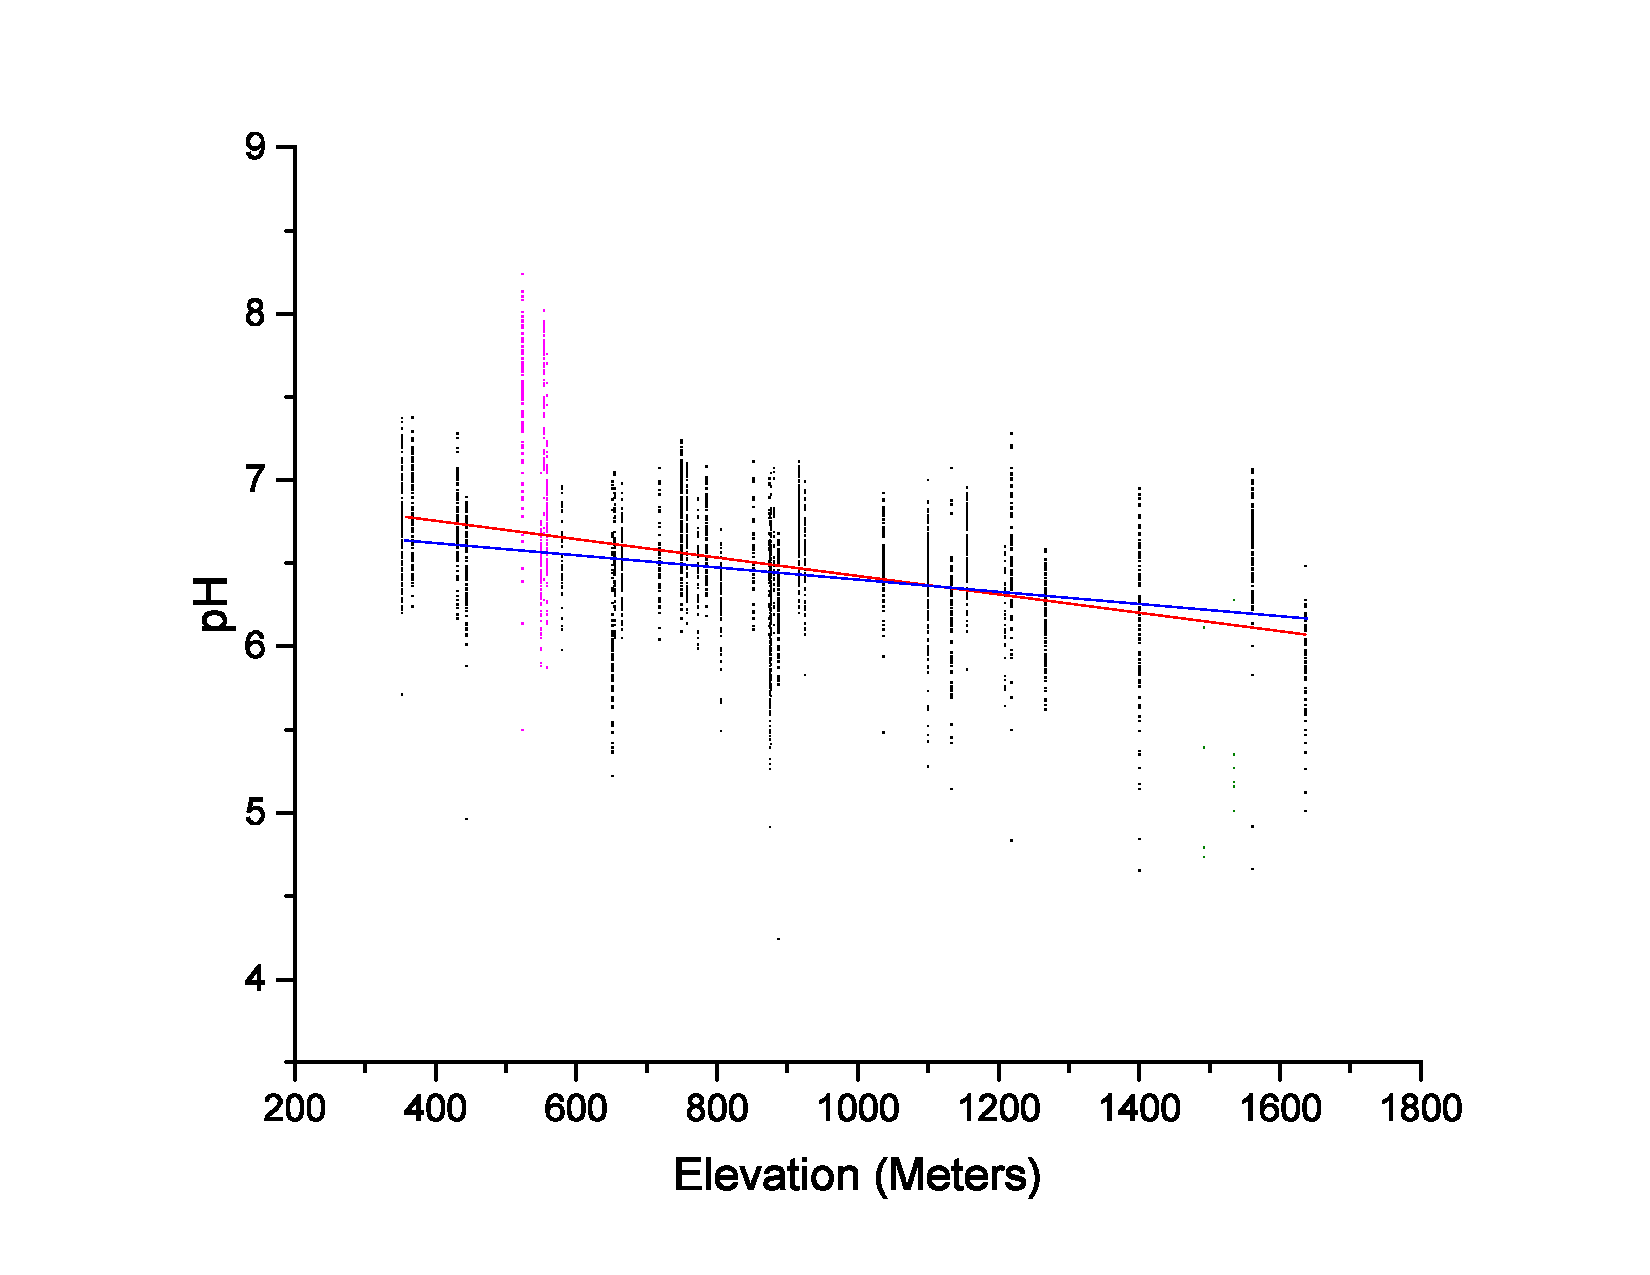
\includegraphics[width=6in]{pHdata}\\
  \caption{pH plotted vs. Elevation.  With and without outliers.}\label{fig:pHdata}
\end{figure}

Several plots were created in order to reduce the variance of the data before any statistical analysis was attempted. JMP was chosen for this task based on its ease of use in plotting data. A plot of pH vs. time visually represents the existence of a positive trend in the pH data from 1993 to 2012.
\autoref{fig:pHdata} shows the pH vs. elevation plot. It shows two trend lines, one which represents the trend of all of the data points and the other represents the trend after the influential points are removed. Both of the trends are negative as elevation increases but the trend line containing the influential points is steeper. pH was plotted against the month that the sample was collected to check for seasonality. Seasonality was expected and found for pH over one year. The variance caused by seasonality will be removed with sine and cosine functions.

Much of the variance in \autoref{fig:pHdata} can be attributed to known influences in the stream survey data: Abrams creek watershed, sites that are affected by anakeesta geology, and stormflow \citep{neff2012influence}.  Comparatively Abrams is a low elevation, low slope area where the underlying geology is Cades Sandstone, which buffers against acid rain very well. This sandstone contributes to high ANC values which in turn keep the mean pH levels higher than the rest of the sites in the survey. Site numbers 237 and 252 are sites which are down hill of road cuts that have exposed the underlying anakeesta formation to runoff. The anakeesta formation contains sulfidic slate ,which can have the same negative effect of acid deposition,  and keeps the pH values of streams very low.

Stormflow is both influential and detrimental  to GRSM water quality. Storms can bring high intensity rain fall which can very quickly reduce the pH and ANC of streams. In streams with low ANC and pH, episodic stream acidification can be harmful to aquatic life \citep{neff2009physiological}.  Stormflow runoff can have a higher contribution to stream acidification than baseflow because it transports protons left in the upper layers of the soil by acid deposition. Stream acidification caused by stormflow can cause base cation exchange through the leaching of the surrounding soil. When the inherent base cation minerals run out, excess H$^+$ and Al will be released into the water. Increasing the H$^+$ concentration will lower the pH, and Al is toxic to biotics. Healthy streams can rebound to normal pH values; unhealthy streams can have permanently lowered ANC due to leaching.  Measurements taken from stormflow can show uncharacteristically low pH values and high amounts of metals from leaching. In this way, stormflow is sometimes considered an influential group on the rest of the data, because the measurements are significantly different from the average. Dr. Cai characterized all of the available water quality data between 1993 and 2010 as storm flow or baseflow; this work is summarized in \citet{cai2012}. Water quality data after 2010 had not been characterized. If all stormflow observations are to be kept in the data, the years 2011 and 2012 would need to be characterized. Quick analyses were run to see how influential stormflow was on the data as a whole, and it turned out that some were and many were not. Instead of throwing out all of the stormflow observations at once, single influential observations could be explained by stormflow and removed. They can be removed on a case by case basis during the regression method.

The regression process includes preparing the data and identifying influential observations. The output of a step-wise regression analysis performed in SPSS can be configured to complete many different analyses in order to smooth the data. The different tests applied for this paper include tests for normality, heteroscedasticity, cook's D, DFBETAS, and DFFITS. As observations were identified by cook's d, DFBETAS, and or DFFITS as influential, they were individually analyzed to determine what made them influential. Modification or removal of an influential observation had to be justified, or it would remain an outlier. An example of modification of the data included a pH value that read 16.47 was changed to 6.47. Another example is that some conductivity values were obvious copies of the ANC value for the same observation. These conductivity values were removed. Some influential observations were not as obvious and if they could not be labeled as storm flow or human error they would be kept. After sufficient attention was given to the influential observations the analysis was re-run and more influential observations could be found, and attention would need be given to these also. This process was completed for all four of the dependent variables, (pH , ANC, NO$_3^-$, and SO$_4^{2-}$).
 
 The step-wise variable selection process requires a list of variables to choose from.  These variables are reported in \autoref{variables}.  The variables chosen for this list were chosen from those chemistry values recorded in the full stream survey dataset.   One benefit of choosing only variables directly from the stream survey dataset is a high ease of repeatability for the future.   The step-wise process regulates entry into the equations by the probability of the F statistic.  If this statistic were between .05 and .10 then the variable could stay.   The variables selected were used to create the fixed models presented in \autoref{tab:stepwiseeq}.  If any of the time variables were chosen by the step-wise method then the others were added.  This was done to ensure the Julian date coefficient was present along with $\sin(\theta)$ and $\cos(\theta)$ for seasonality.  Many variables are present in the stream survey database, some are measurements but others were derived.  Mathematically seasonality can be modeled with the $\sin(\theta)$ and $\cos(\theta)$ variables as shown in \citet{helsel1992statistical}.  They represent each day of the year as a fraction of the year and place the lowest pH on January 1 and the highest on July 1.  The variable BC (base cations) represent the sums of the Ca$^{2+}$, Mg$^{2+}$, K$^+$, and Na$^+$ measurements.  Correlations were run between each of the proposed variables  and both ANC and BC were found to be better described as $\log_2(ANC)$ and $\log_2(BC)$.
 
\begin{table}[htbp]
\caption{Equations created through step-wise variable selection}
\begin{tabular}{lp{7.5cm}cc}
\toprule
Dependent (n)     &Model                                                                                                                                                                                                                                                                                                                                                                                                       & Adjusted $r^2$  & Model p \\ 
\midrule
pH (3116)            &$.673\times\log_2(\text{Sum Base Cations}) + (-.368\times \text{NO}_3) + (.262\times \text{Julian Day}) + (-.266\times \text{SO}_4) + (-.050\times\cos(\theta))$                                                                                                                                       & 0.630                  & $<$0.001 \\
ANC (3116)         &$ (.415\times \text{Sum Base Cations}) + (-.185\times \text{SO}_4) + (.595\times \text{Conductivity}) + (-.102\times \text{NO}_3) + (.019\times \text{Julian Date}) + (.005\times \text{Cl}) + (.005\times \sin(\theta))$                                                & 0.984                  & 0.049 \\
NO$_3$ (3116)   &$(-.295\times \text{SO}_4) + (-3.183\times \text{ANC}) + (2.19\times \text{Conductivity}) + ( .923\times \text{Sum Base Cations}) + (.120\times \text{Julian Date}) + (.051\times \text{Cl}) + (.047\times \sin(\theta)) + (.031\times \cos(\theta))$ &0.498                   & 0.017 \\ 
SO$_4$ (3116)   &$ (-.166\times \text{NO}_3) + (2.318\times \text{Conductivity}) + (-3.229\times \text{ANC}) + (1.033\times \text{Sum Base Cations}) + (.042\times \text{Julian Date})$                                                                                                                               & 0.720                  & $<$0.001 \\ 
\bottomrule
\end{tabular}
\label{tab:stepwiseeq}
\end{table}
%these two paragraphs need work
 The difficulty in modeling a time trend is the high amount of variation within the datasets.  While trying to determine a time trend other variables are added besides those that explain a trend in time. All of the equations contain the time variables (julian date, $\sin(\theta)$, and $\cos(\theta)$) along with the chosen chemical variables.  Because of the difficulty of explaining what the Julian date coefficient really means along side the chemical variables a second set of equations was created for analysis.  Theses equations use only the three time variables to describe each of the dependents.
 
 Elevation was not a significant predictor for any of the dependent water quality variables chosen.  The dependent variables were regressed using simple linear regression against elevation in meters in order to determine their trends by elevation.  These trends encompass all elevations; no elevation bands were used.
 
\section{Results}

Julian date coefficients are are reported in \citet{robinson2008ph} for each of the eleven historic elevation classes and across each of the dependent variables (pH, ANC, NO$_3^-$, and SO$_4^{2-}$).  Julian date coefficients for this paper were reported in similar tables.  144 different Julian date coefficients were calculated and are presented in two tables.  \autoref{tab:Step-wise julian date} records the Julian date coefficients calculated using the equations in \autoref{tab:stepwiseeq}  and \autoref{tab:time vars} records the Julian date coefficients for  equations containing only the three time variables.  Each trend line is represented by its Julian date coefficient, the $r^2$ value for the trend line, and it's statistical significance.

2 of the 72 trend lines in \autoref{tab:Step-wise julian date} are insignificant.  In contrast 50 of the 72 trend lines in \autoref{tab:time vars} are insignificant.   Setting the linear regression $\alpha$ at .05 forces any trend with a p-value greater than .05 to be insignificant.  Insignificance rejects the hypothesis that $\beta$(the coefficient) $\neq 0$.  A p-value greater than .05 means that there is greater than a 5$\%$ chance that $\beta=0$ or in this case the Julian date coefficient =0. 

\subsection{Step-wise Julian date coefficients}

\subsubsection{pH}

The Julian date coefficients In \autoref{tab:Step-wise julian date} for pH showed negative time trends in three statistically significant regression lines, all in the time range of 1993-2002.  These lines were in elevation classes 2, 3, and 5.  There is one degrading trend in the third time set (2009-2012) and in the fifth elevation class but it is insignificant.   Most of the trend lines report that pH is increasing over time.

\subsubsection{ANC}

Trends for ANC fluctuate while evaluating across time sets and elevation classes .  Eleven of the lines are positive, and seven are negative.   Two of the three negative trends for ANC in set 2 have a smaller slope in set 3, and one of the degrading trends in set 2 becomes positive in set 3.  When comparing time set 2 to set 3, ANC trends are growing over time. 

\subsubsection{Nitrate}

NO$_3^-$ trends in set 2 are all positive. In set 3 NO$_3^-$ has a decreasing trend  in elevation class 4. The NO$_3^-$ trends for set 1 are half positive and half negative. But from the years 2003 to 2008 all of the NO$_3^-$ trends are positive. In set 3, the trend in elevation class 4 has a negative trend.

\subsubsection{Sulfate}

SO$_4^{2-}$ has mixed positive and negative trends for set 1 but all positive trends for set 2. Half of the SO$_4^{2-}$ trends in set 3 are negative ( 1, 3, and 6).

\subsection{Julian date coefficients from time variables only}

In \autoref{tab:time vars} only 20 of the 72 regression lines are significant, those that have acceptable p-values less than .05.

\subsubsection{pH}

The dependent variable pH in set 1 has zero significant lines, set 2 and 3 combined are slightly less than half insignificant trend lines. The insignificance of the trend lines leaves them untrustworthy, but the trend values themselves are quite similar to those calculated in \autoref{tab:Step-wise julian date}.

\subsubsection{ANC}

There are only two significant regression lines in for ANC in \autoref{tab:time vars}. Elevation class 5 in set 1 has a decreasing trend at -.148, there are no significant lines in set 2 and set 3 elevation class 5 has a positive trend at .891.

\subsubsection{Nitrate and Sulfate}

NO$_3^-$ and SO$_4^{2-}$ both had negative trends in set 1 class 1. These are the only significant decreasing trends exhibited for either NO$_3^-$ or SO$_4^{2-}$  in \autoref{tab:time vars}.  Both have positive trends in set 2 at elevation classes 1,2,4 and 6, and neither variable have significant lines in set 3.

\subsection{Elevation trends}
\begin{table}[htbp]
\centering
\caption[Elevation trends]{Dependents regressed against elevation (m) only.}
\begin{tabular}{llcccc}
\toprule
set & Dependent & n & slope&$r^2$&per +1000m \\ 
\midrule
1   & pH               & 1357 & .000 & .173 & -0.411  \\ 
     & ANC            & 1354 & -.056 & .199 & -56.227  \\ 
     &  NO$_3^-$ & 1161 & .032 & .372 & 32.211  \\ 
     &  SO$_4^{2-}$& 1343 & .037 & .108 & 37.371  \\ 
     & SBC             & 1358 & .013 & .005 & 13.065  \\ 
\midrule
2   & pH               & 997 & .000 & .094 & -0.391  \\ 
     & ANC            & 997 & -.051 & .157 & -50.970  \\ 
     &  NO$_3^-$  & 995 & .031 & .307 & 30.677  \\ 
     &  SO$_4^{2-}$ & 1029 & .036 & .098 & 35.793  \\ 
     & SBC             & 1031 & .016 & .009 & 15.537  \\ 
 \midrule
3   & pH              & 757 & .000 & .061 & -0.286  \\ 
     & ANC           & 757 & -.036 & .087 & -35.689  \\ 
     &  NO$_3^-$ & 757 & .026 & .195 & 25.924  \\ 
     &  SO$_4^{2-}$ & 757 & .030 & .101 & 29.715  \\ 
     & SBC            & 757 & .020 & .014 & 19.905  \\ 
 \bottomrule
\end{tabular}
\label{tab:Water quality per elevation}
\end{table}

The aim of \autoref{Water quality per elevation} is to calculate the change in water quality values for every 1000 meters of elevation.  The base cations were added as a dependent for this analysis.  All of the pH and ANC values decrease as elevation increases and all of the  NO$_3^-$ , SO$_4^{2-}$ , and base cations dependents increase as elevation increases.  Every value in the right most column decreases for the water quality dependents as the table moves forward in time sets except for the base cations .

\subsection{Results by Comparison}

In comparing table 4 from \citet{robinson2008ph} with \autoref{tab:Step-wise julian date} from this study, it needs to be noted that the elevation classes are different and the data sets have slightly changed throughout the years. The largest difference is the reduction of 90 sites to 43. Abrams was not included in this analysis but was included in \citet{robinson2008ph}. This difference could explain the differences seen in the old elevation classes from \citet{robinson2008ph} of 1,2, and 3 and elevation class 1 in this study. Two sites (237, 252) that are in the new elevation class 6 were left out of the statistical analysis as influential observations. These correspond to historic elevation class 9.

One interesting comparison between table 4 of \citet{robinson2008ph} and set 1 of this study are the differences in pH coefficients. All of the pH trends presented in table 4 of \citet{robinson2008ph} are negative which is what led to the statements that pH is dropping and can continue to dangerous levels in the future. However, only half the time trend trends for set 1 for pH found in this study were negative in \autoref{tab:Step-wise julian date}. All of the rest of the pH trends for Julian date for both trend analyses are positive when they are significant.

\paragraph{pH and ANC}
For a data set of 92 sites within the time frame of 1993 to 2009 \citet{cai2012} reports a decrease for pH and ANC of -0.32 pH units and -35.73 $\mu$eq L$^{-1}$ per 1000-ft elevation gain or 302-m elevation gain respectively.  These values are close to those found in this study for the years of 2009-2012, but the slopes in set 1 and 2 are much steeper.  In set 3, pH is significantly lower with a trend of -.0286 pH units per 1000-m gain and ANC is a little bit lower with a trend of -35.689 $\mu$eq L$^{-1}$ per 1000-m gain(\autoref{Water quality per elevation}).  

\paragraph{Nitrate and Sulfate}
The positive SO$_4^{2-}$ trends seem to decrease by 2 $\mu$eq L$^{-1}$ between set 1 and set 2 in \autoref{Water quality per elevation} and then by 6  $\mu$eq L$^{-1}$ between set 2 and 3.  In contrast, an insignificant negative trend with elevation was found in \citet{cai2012} for the years 1993 to 2009.  NO$_3^-$ follows a similar pattern as SO$_4^{2-}$ in \autoref{Water quality per elevation} which is also in agreement with findings in \citet{weathers2006}.  As the trends for  NO$_3^-$ and SO$_4^{2-}$ decrease over the time sets the base cations increase by 2 $\mu$eq L$^{-1}$ between set 1 and set 2 and then by almost 5 $\mu$eq L$^{-1}$ between set 2 and set 3.

\section{Discussion}

It is interesting that the step-wise process did not choose elevation as an independent variable for any of the dependent variables. \autoref{fig:pHdata} clearly shows a decreasing trend for pH while increasing the elevation. Individual elevation classes might be to small to show a significant elevation trend.  Increasing acidification with increased elevation was observed in \citet{cai2012} will analyzing the entire 1993 to 2009 dataset available.  This suggests that there is an elevation trend it is just not as important as other factors when studying acidification in the GRSM.% could get some comparative analysis in keil's basin paper

A trend in time is also clearly evident with a simple plot of pH vs. time but the mostly insignificant trends of \autoref{tab:time vars} suggest otherwise. The three time variables alone are not enough to explain the dependent variables.  \citet{robinson2008ph} found that pH was decreasing over time when looking at stream survey data between 1993 to 2002, although this study found that most of the trends in that period are negative, the trends for 2009 to 2012 are all positive as well as the trends for 2003 to 2008.  This is in agreement with values reported in \citet{cai2012}.  The differences between the results in \citet{robinson2008ph} and those in \autoref{tab:Step-wise julian date} and \autoref{tab:time vars} imply that water quality is worse in the past but is getting better.  Both \citet{robinson2008ph} and \citet{cai2012} used more than double the sites of this study and \citet{robinson2008ph} allowed Abrams to stay in the data.  The differences in the data can account for differences in the results but it is safe to say that water quality in the park is getting healthier.

SO$_4^{2-}$ has more decreasing trends for the years 2009 to 2012 than in any other time set. This is not surprising based on the values shown in \autoref{fig:sulfateemissions} in which SO$_4^{2-}$ concentrations at the high elevation site Noland begin to drop along with emissions from Kingston and Bull run power plants.  It is surprising that \cite{cai2012} found an insignificant but negative trend in SO$_4^{2-}$ as elevation increases while this study shows only increasing elevation trends for all time sets.  When looking at a graph of SO$_4^{2-}$ vs. elevation there are many higher elevation outliers present, these outliers could make the difference in findings.%graphs?

Water quality is increasing.  pH and ANC are rising and the pollutants NO$_3^-$ and SO$_4^{2-}$ are decreasing.  The concerns of lowering pH raised in \citet{robinson2008ph} are now not as important as those for SO$_4^{2-}$ desorption raised in \citet{cai2012}.  The lack of elevation trend in SO$_4^{2-}$ was attributed to high elevation soil adsorption of depositional SO$_4^{2-}$ and a statement was made that SO$_4^{2-}$ remains absorbed to soil particles as long as soil water chemistry remains high in SO$_4^{2-}$ concentration and low in pH \citep{cai2011long}.  The slope for the elevation trend of SO$_4^{2-}$ over the three sets is decreasing but most of the mean SO$_4^{2-}$ concentrations listed in \autoref{tab:Descriptive Statistics} are increasing through time along with pH.

The advantage of using regression for trend analysis is its prediction abilities but regression is more difficult than the nonparametric methods of trend analysis.  Tests for normality and heteroscedasticity along with variable transformations take care of forcing the usually nonparametric water quality data to be parametric.  Nonparametric tests are more robust and do not require as much preparations to run and in the end are more reliable.  \citet{robinson2008ph} predicted negative trends and 9.4 years for the historic elevation class between 914 and 1067 meters to reach a ph of 6.00.  This corresponds exactly to this study's elevation band 4 which received an increasing pH trend in all three time sets.  The differences being the sites used and the equations formed through the step-wise process.  The equations in \citet{robinson2008ph} follow the theory behind acidification much more closely where as the equations created in this study used variables already  available in the running stream survey dataset.  Prediction is hard and unless it is absolutely necessary to use then the Mann-Kendal test for trends would be much easier, more reliable and more robust \citep{helsel1992statistical}.      
